\documentclass[12pt]{article}
\usepackage{iftex}
\usepackage{graphicx}
\usepackage{enumitem}
\usepackage{hyperref}
\usepackage[style=apa, backend=biber]{biblatex}
\addbibresource{phd_bombus.bib}
\setcounter{maxnames}{20}
\setcounter{minnames}{1}
\usepackage{color}
\usepackage{amsmath}
\usepackage{amssymb}
\usepackage[export]{adjustbox}
\usepackage{verbatim}
\usepackage{mathpazo}
\usepackage{setspace}
\usepackage{multirow}
\usepackage{lscape}
\usepackage{fancyhdr}
\usepackage[normalem]{ulem}
\usepackage{rotating}
\usepackage{chngcntr}
\usepackage{float}
\usepackage[parfill]{parskip}
\usepackage[tiny,compact]{titlesec}
\usepackage{longtable}
\usepackage{textcomp}
\usepackage{rotating}
\usepackage{xr}
\usepackage{caption}
\usepackage{siunitx}
\usepackage[T1]{fontenc}
\usepackage{gensymb}
\sisetup{round-mode=places, round-precision=2, detect-all}

\newcommand{\flagged}[1] {
  \textcolor{blue}{#1}
}

\hypersetup{colorlinks=true, linkcolor=black, citecolor=black}
\RequirePackage{lineno}

\renewcommand{\thefigure}{A\arabic{figure}}  % Prefix figures with "S"
\setcounter{figure}{0}  % Reset figure counter
\renewcommand{\thetable}{A\arabic{table}}
\setcounter{table}{0}
\setcounter{section}{0}

\def\title{Appendix 1 -- Population Genetics and Colony Assignments}



\begin{document}
\begin{center}
  {\large \title \par}
\end{center}\par

\section{Assessing locus $F_{is}$, $F_{st}$ and linkage disequilibrium}

\begin{figure}[H]
    \centering
    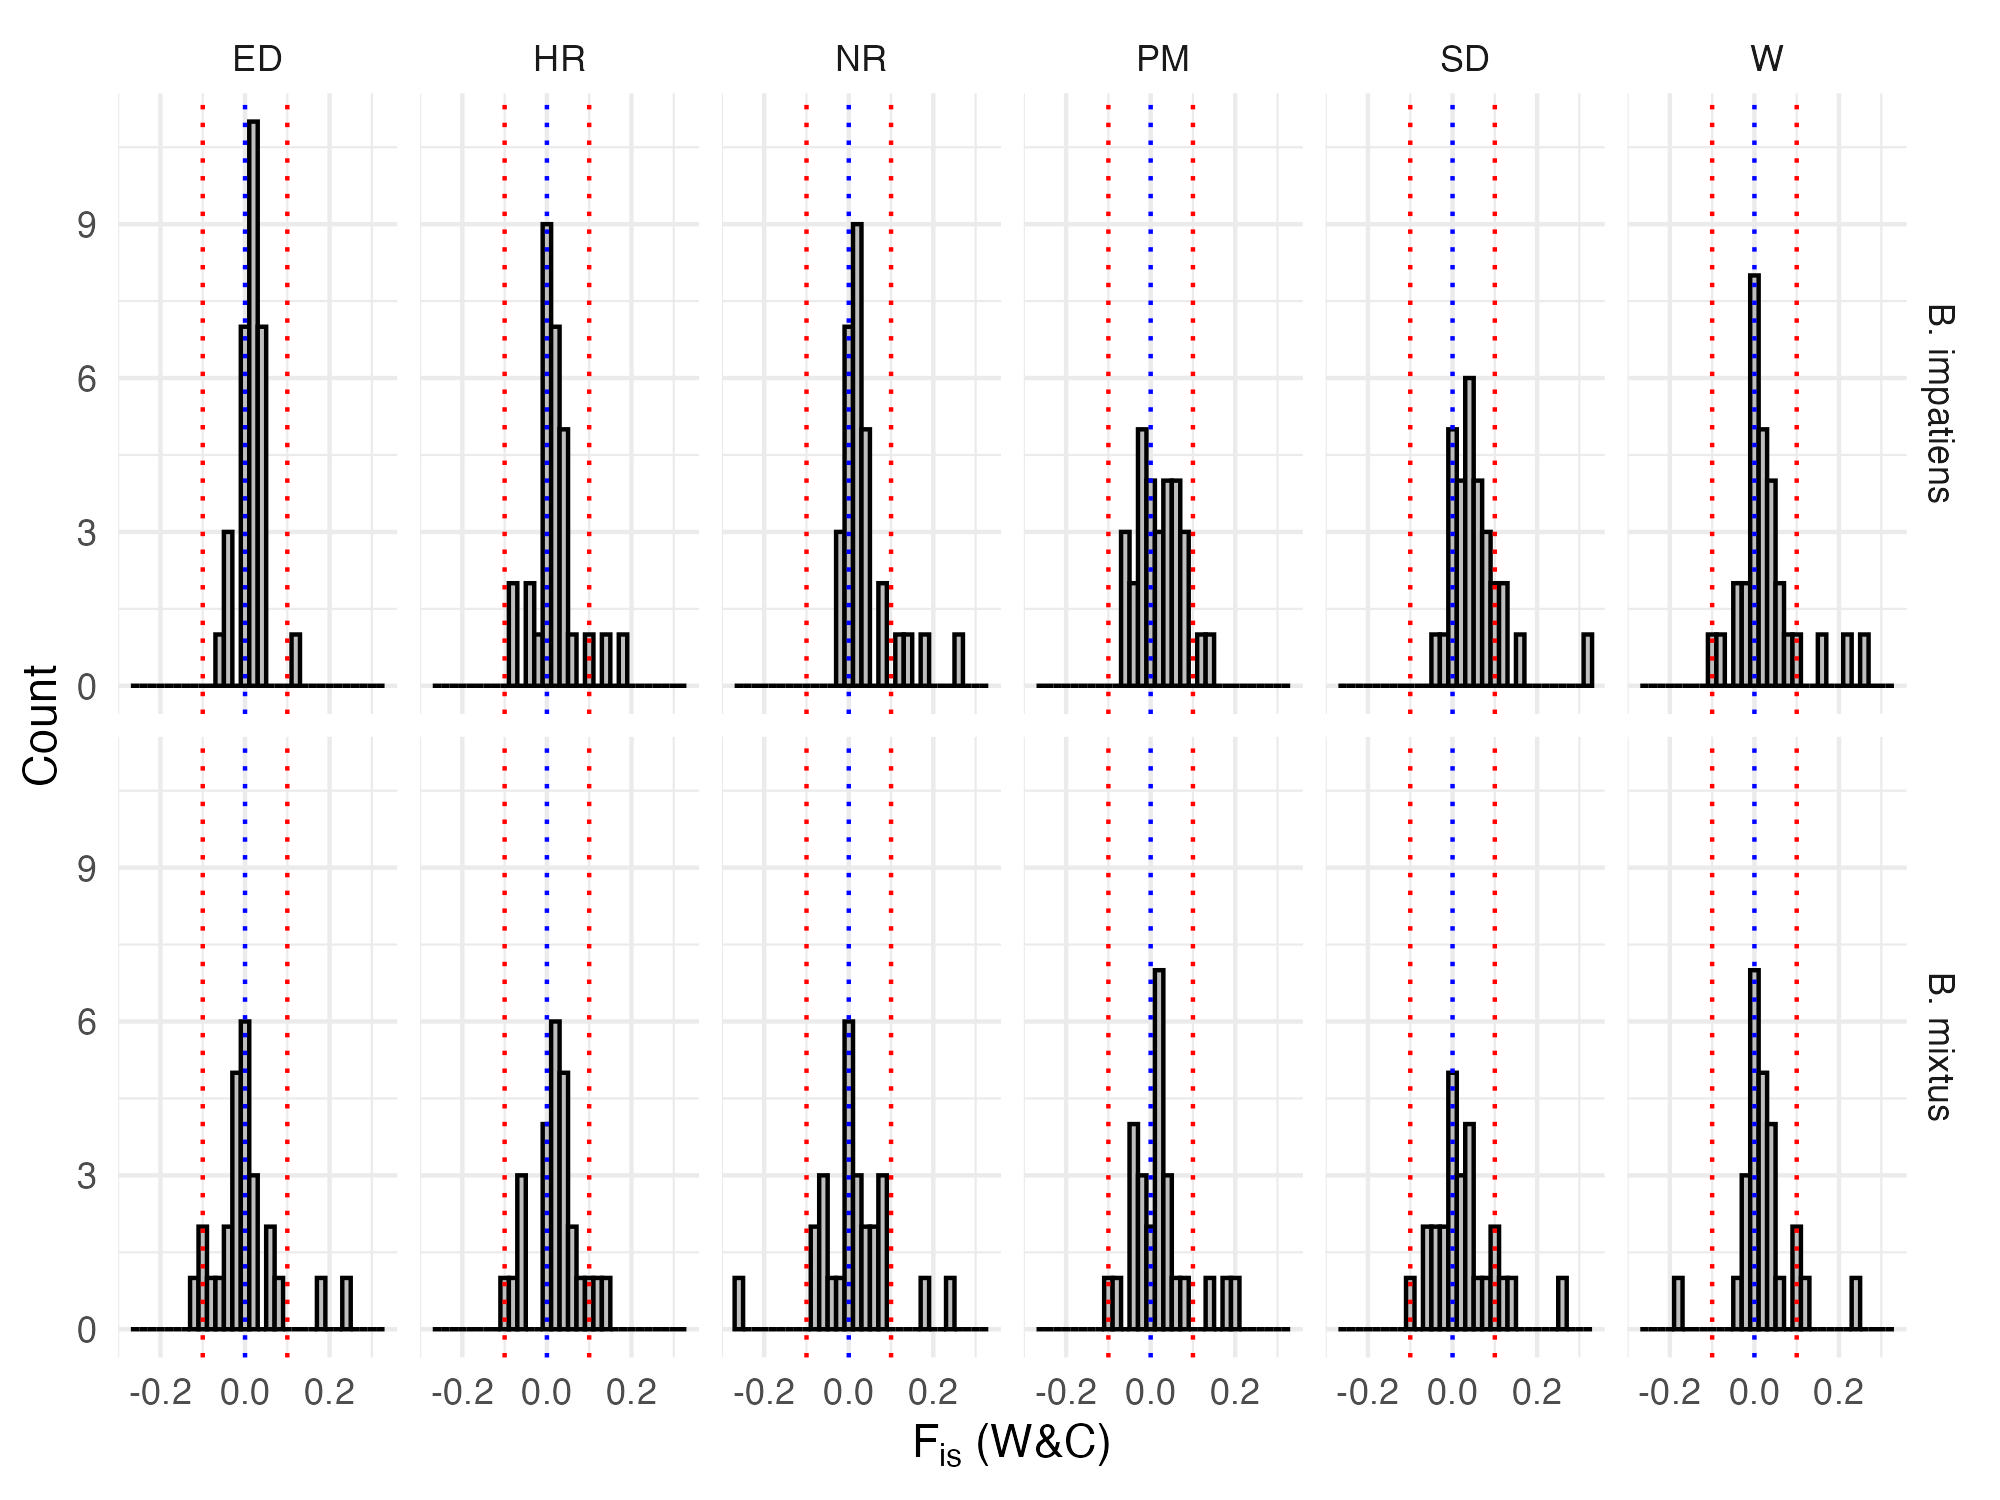
\includegraphics[width=\linewidth]{appendix_figures/Fis.jpg}
    \caption{Estimates of $F_{is}$ for each locus in each subpopulation. Estimates from 2022 and 2023 were calculated separately but are shown together for each site x species combination. Blue dotted lines indicates $F_{is} = 0$ and red dotted lines indicate $F_{is} = \pm 0.1$.}
    \label{fig:Fis}
\end{figure}


\begin{figure}[H]
    \centering
    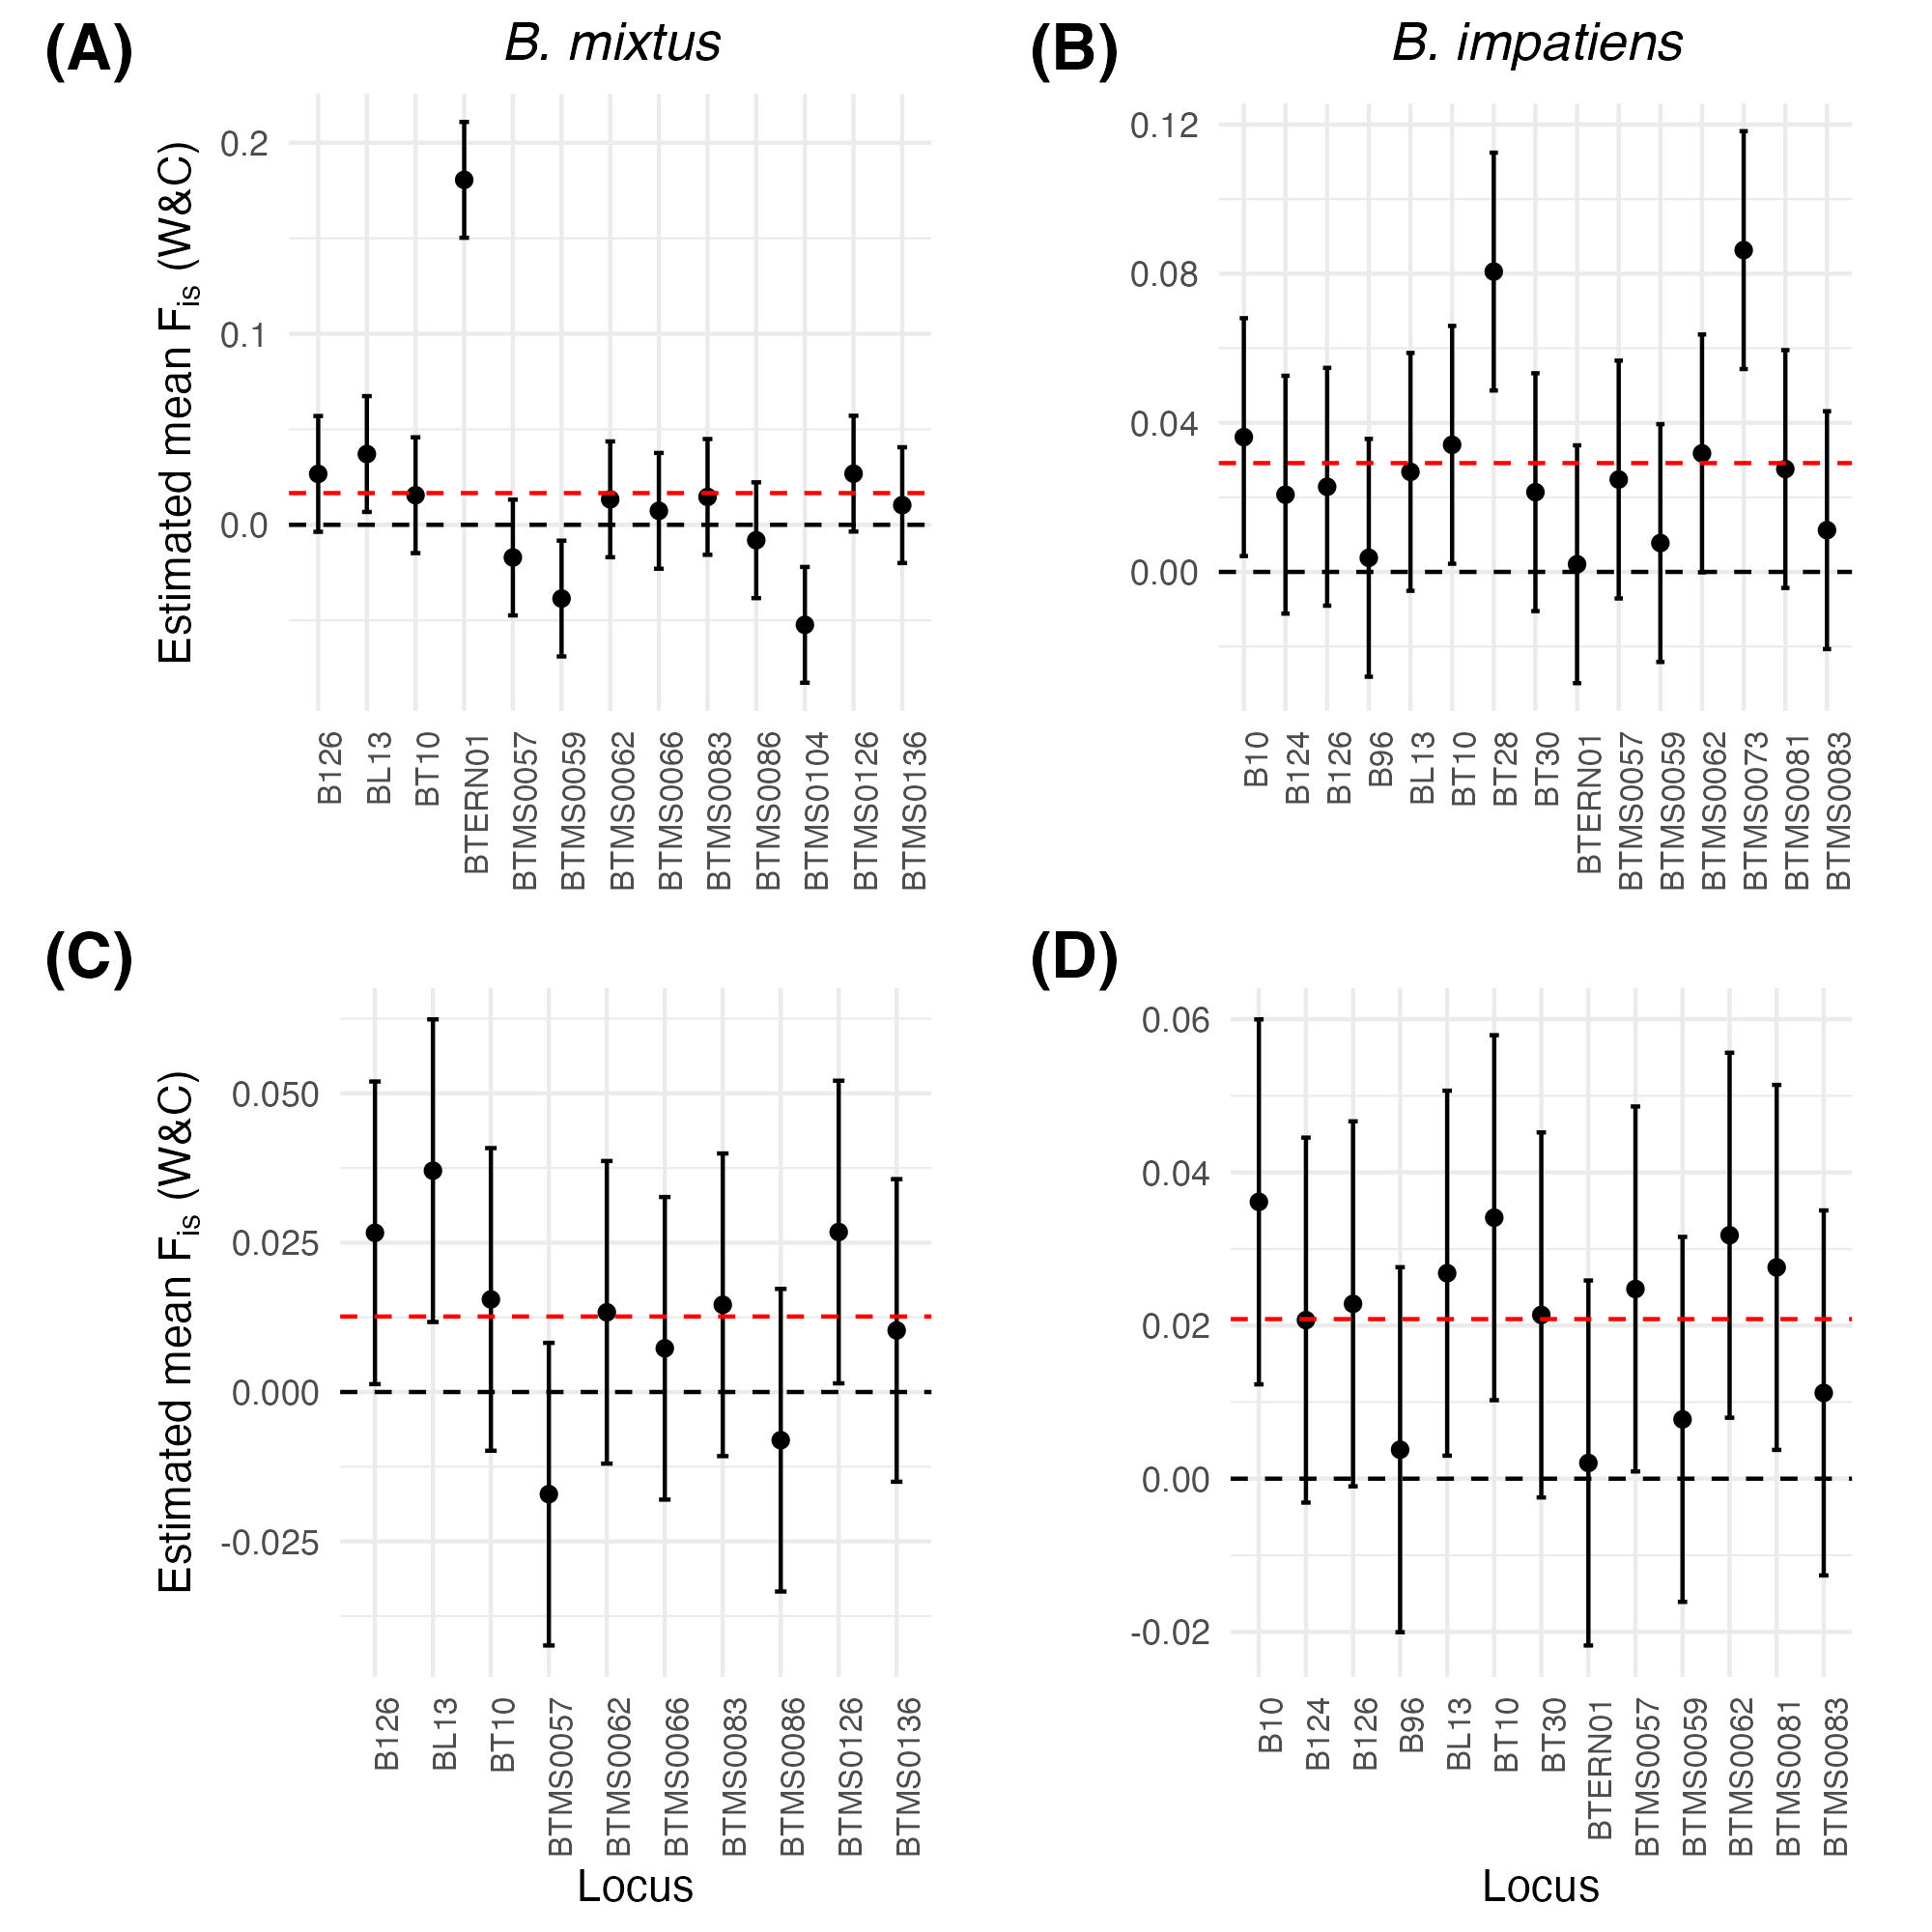
\includegraphics[width=\linewidth]{appendix_figures/marginalmeans.jpg}
    \caption{Locus-specific $F_{is}$ marginal means. A) \emph{B. mixtus} all loci; B) \emph{B. impatiens} all loci; C) \emph{B. mixtus} loci following iterative removal of loci which differed significantly from global mean $F_{is}$; D) \emph{B. impatiens} loci following iterative removal of loci which differed significantly from global mean $F_{is}$. Dashed black line denotes $F_{is} = 0$, dashed red line denotes global mean $F_{is}$ for each species.}
    \label{fig:marginalmeans}
\end{figure}


\begin{figure}[H]
    \centering
    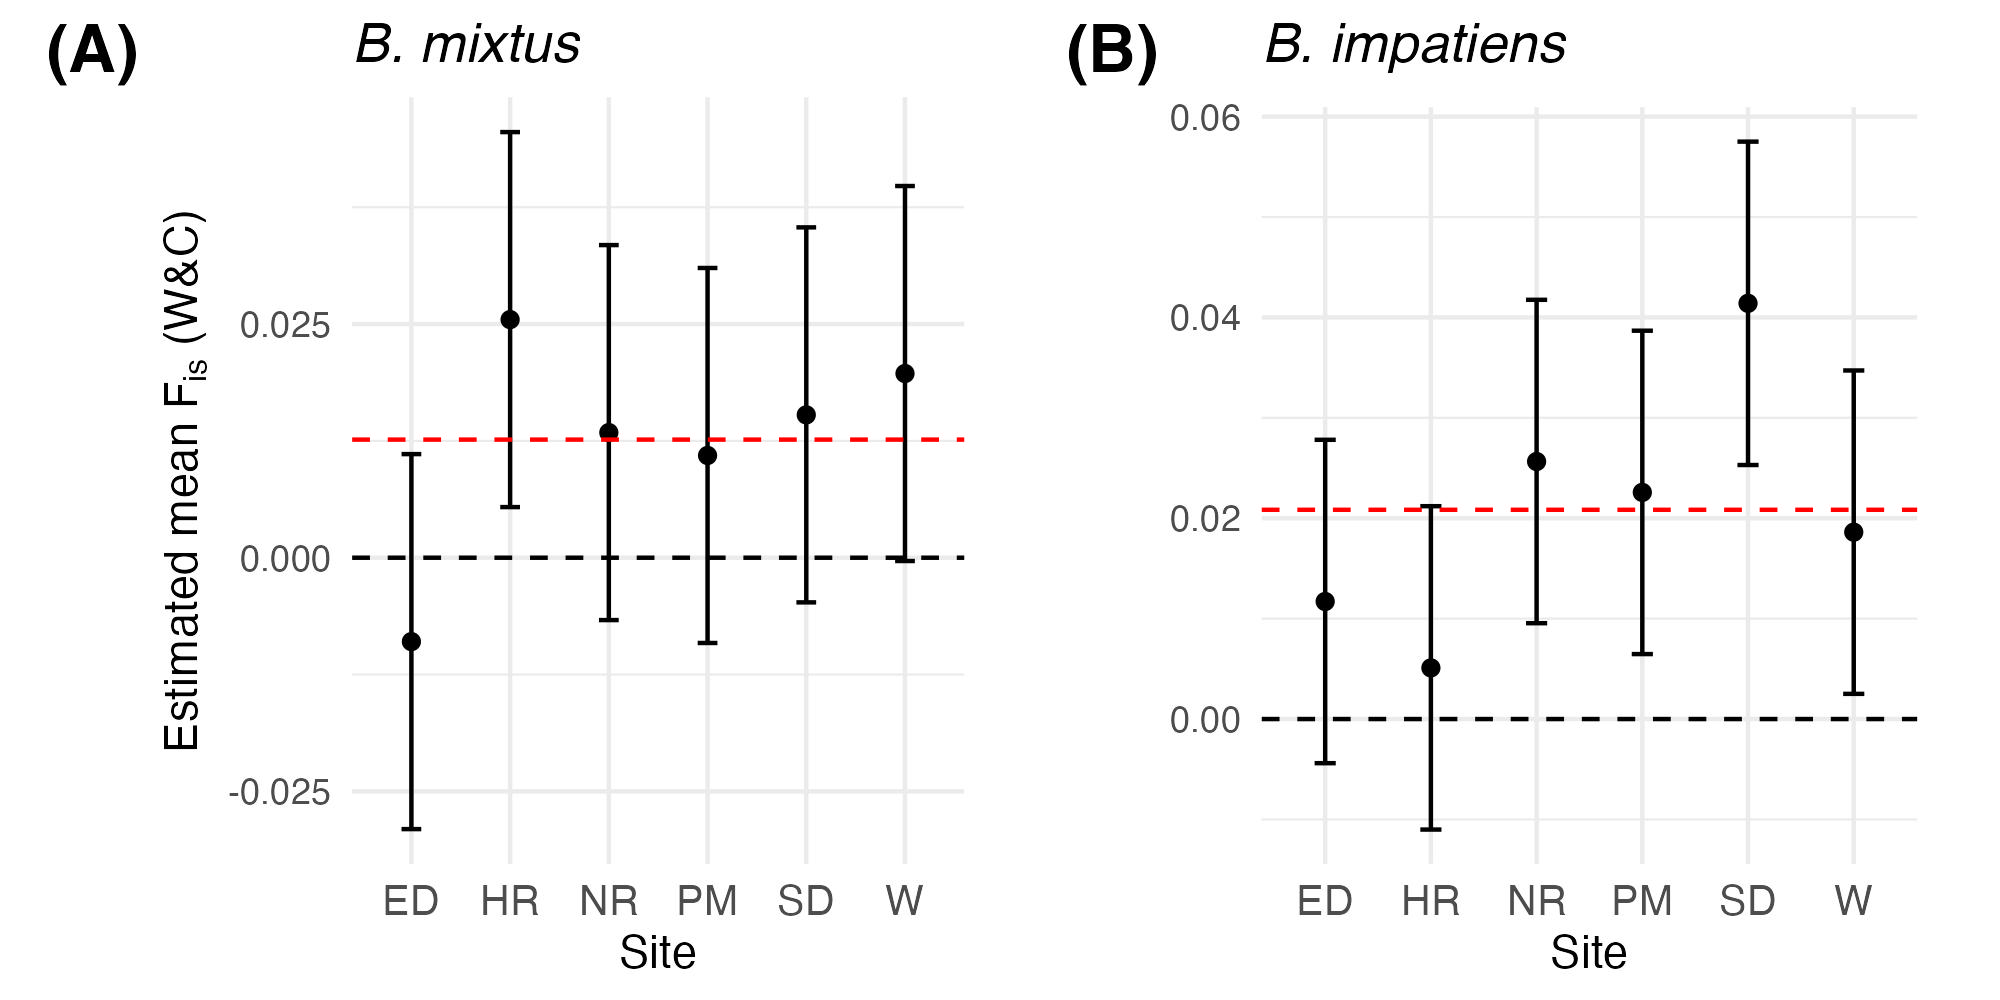
\includegraphics[width=\linewidth]{appendix_figures/siteFis.jpg}
    \caption{Site-specific $F_{is}$ marginal means following removal of low-quality loci for A) \emph{B. mixtus} and B) \emph{B. impatiens}. Dashed black line denotes $F_{is} = 0$, dashed red line denotes global mean $F_{is}$ for each species.}
    \label{fig:siteFis}
\end{figure}


\section{Testing COLONY on simulated data}


\section{Observing colonymates at multiple sites}


\end{document}